\chapter{Vision}

\section{Working Process}
\subsection{Overview}

We began our project by getting familiar with ROS, doing many tutorials on it and setting everything up. Then we learned a lot about Kinect, its function and its possible applications. Further we started integrating ar\_track\_alvar – AR tag tracking library -  in ROS, installed and calibrated it and got rid of all possible errors. \\
\begin{figure}
\begin{center}

\includegraphics[width=\linewidth]{graphics/markers.png}
\caption{Few marker examples}
\label{Few marker examples}
\end{center}
\end{figure}
From this moment and later on, we ran into all sorts of problems and bugs. We spend a lot of time fixing them and finding a right solution to every single problem. To get the best result of the marker recognition we tried bundle of markers as well as one single marker (we were limited by the size of an A4 page) and tested the Kinect's field of view, i.e. how far away it can see the marker and which angle can be maximally reached so that Kinect still recognizes the marker. We generated markers and when its detection and recognition were correctly functioning, we started working on getting the right data from ar\_track\_alvar and learned how to interpret this data in ROS. Then we used it to get the world coordinates according to the coordinates of the robot and to get the covariance. Afterwards we put our hands on the Pan-Tilt Unit, device used for head movement. We spend time installing PTU drivers on computer and configuring it, got familiar with basics of PTU movement and tried to design an efficient algorithm to move the head towards seen marker. Later on we came to the last step: we implemented the function, that tells other groups information about next expected marker. After that we generated all the markers and put it on walls according to the map of the building,with the right distance from each other, and created a database for all the markers. Finally, at the end, we tested written software and got rid of every found error and bug.

\subsection{Tasks assignment}

Starting from October we worked hard to achieve our goals. We had a lot of unexpected as well as expected problems, most part of them helped us to acquire new knowledge, but some of them just took a lot of time to solve. Our team was formed out of three people. Guilherme Pires is gone and he made his contribution to the documentation separately by writing in the wiki page, so his work will be only briefly discussed here. From the beginning we divided all our incoming tasks equally in the group, so that everyone could make a good contribution to the project. In the following chapter will be explained differentiation of tasks in the group. Guilherme Pires has brought good knowledge in Linux system with him, the rest two of us needed to learn it at first. As we started working on ar\_track\_alvar, Guilherme and Valeriy integrated it in ROS environment and set it up. At the same time Codrin worked on the data processing from ar\_track\_alvar, learned a lot about TF-Trees and ar\_track\_alvar itself. Later on he created an algorithm to change the coordinates from the marker, that we get from ar\_track\_alvar to the world coordinates and publish them to the other groups. Meanwhile Valeriy calibrated the marker recognition, generated markers and worked himself through all sorts of errors delegated him from other teammates. Later on Guilherme implemented algorithm for computation of the covariance. Valeriy started working on tracking markers with the Pan-Tilt Unit, challenged with problems like finding an appropriate mathematical function to implement the movement, calibrating the turning speed, working on a problem with stopping the head on time, and at then testing and debugging it. Almost at the end we worked on the next expected marker problem, discussed the details and all possible solutions, made then a concept algorithm, that was implemented later on by Guilherme and Codrin. Then Valeriy was dealing with testing of all the software, writing a testing program and resolving appeared errors.  Meantime Codrin concentrated on unexpectedly appeared problem with computation of coordinates, which he successfully fixed.  

\subsection{Used Resources} 

We used a lot of open source resources, that were essential to our success. From the beginning we learned a lot about Linux, because we hadn’t had much experience in it. Then we became familiar with ROS, its packages, nodes, core commands and its functioning principle in general. We learned all the concepts starting from catkin and roscore, all the way up to tf and so on. As a visualisation and debugging tool rviz was very helpful for checking for example if axes direction were right. rqt\_graph helped us understand connection between different nodes. We successfully applied Kinect in our work with markers recognition, which were generated with ar\_track \_alvar - an open source AR tag tracking library for ROS. “createMarker” - another useful tool as part of ar\_track\_alvar, that helped us to create graphical representation for bundle of markers as well as for single marker and each time generate XML file for it. Later on, when we started working with Pan-Tilt Unit in purposes of the head movement, we installed flir\_ptu\_driver, ptu46 and ptu\_control in order to be able to control the PTU.

\section{Conceptual Design}

\subsection{Components}
At a conceptual level, Vision package can be decomposed in two components, implemented in two ROS nodes: localizer and marker\_broadcaster. The internal interaction between them and all other external nodes does not need to be understood or changed from the exterior, as the whole setup is launched in the custom vision.launch file of the package Vision.
The marker\_broadcaster node is responsible for feeding the tf system with the position of all markers inside the database. Localizer, as the node with the main functionalities, deals with the processing of data from the Kinect camera and uses the tf data from marker\_broadcaster in order to output a position with covariance. The data flow inside the Vision package node undergoes the following transformations in order to output the position of the camera:


\begin{figure}[h]
\begin{center}
\includegraphics[width = \linewidth]{graphics/vision_concept.png}
\caption{Vision Concept}
\label{The transformations which data undergoes from input to outpout}
\end{center}
\end{figure}

Since the navigation will only take place in one plane which the robot will never leave, all the 3D data is filtered out as soon as possible to keep computations at the appropriate level to avoid computation of unnecessary data. This takes place immediately after the interpretation of the marker position coming from ar\_track\_alvar. From now on in the whole system coordinates will only have 3 values, namely x coordinate, y coordinate, and rotation around z axis. 

\subsection{Dependencies}
The main purpose of the Vision group is to collect data coming from the Kinect camera, process it and output a data in form of a position on the map. The other, less important purposes are the signalization of a seen marker, signalization of an unexpected marker, as well as commands to the Pan-Tilt Unit rotation in order to rotate the head towards the seen or expected marker. In other words, the role that the vision package plays is to serve as a mediator between external ROS nodes feeding it with raw data and generate useful data for the Kalman and High Level Components to process. In order to be able to work, all external dependencies need to be present when being launched. At a conceptual level, these dependencies are:

\begin{enumerate}
\item External ROS packages publishing from outside the project:
\begin{itemize}
\item freenect\_launch for collecting data from the Kinect camera
\item ar\_track\_alvar for processing image data from freenect\_launch and output marker positions
\item flir\_ptu\_driver for managing camera rotation
\end{itemize}
\item Internal ROS packages publishing from inside the project: 
\begin{itemize}
\item High Level
\item Kalman
\end{itemize}
\item Marker positions database in form of a text file.
\end{enumerate}

\subsection{Interactions with other Groups}
Information between the Vision package and the other components of the project is done using the standard ROS messages. The main node from the Vision package publishes pose information coming from higher level nodes of Kalman and High Level group and subscribes to the incoming processed data coming from them.

\begin{description}
\item Output topics:
\begin{itemize}
\item vision/estimated\_pose topic: main topic, in which the position of the robot with respect to world coordinates is published
\item vision/sees\_marker topic: is publishing only when a marker has been seen. 
\item vision/unexpected\_marker  topic: it is intended to serve as a trigger to High Level group in order to signalize that a kidnapping might have occurred.
\end{itemize}
\item Input topics:
\begin{itemize}
\item HL/is\_kidnapped topic: when the signal passed is high, the camera rotation enters a searching state, where it is constantly spinning in search of a new marker
\item kalman/fused\_pose topic: represents the final estimate of the robot position and is used in the computation of the next expected marker in case the HL/is\_kidnapped is on low. By knowing the estimated position, the location of the nearest marker can be computed and in case nothing is seen, the camera rotates towards that direction.
\end{itemize}
\end{description}

\section{Implementation}

\subsection{Input/Output Specification}
The Vision package communicates with other ROS nodes exclusively through topics. There are input and output ports, local topics that stay within the project to communicate with other teams, and global topics that go outside the project to reach for data input and to send commands.

\begin{itemize}
\item geometry\_msgs::PoseWithCovarianceStamped: output internally to topic “vision/estimated\_pose”. Represent the main functionality of the vision package, i.e. to provide global robot coordinates computed from camera input and marker database.
\item std\_msgs::Bool: output internally to topic “vision/sees\_marker”. Is publishing true whenever a marker is identified by the Kinect camera.
\item std\_msgs::Bool: output internally to topic “vision/unexpected\_marker”. Is publishing whenever the position it receives from Kalman group does not match with the currently seen marker
\item std\_msgs::Bool: input internally from topic “HL/is\_kidnapped”. Used to decide the camera rotation strategy: whether it shall rotate in search of a marker, or rotate towards expected marker on the map.
\item geometry\_msgs::PoseWithCovarianceStamped: input internally from topic “kalman/fused\_pose”. Used to determine the distance, direction and finally ID of the next expected maker.
\item ar\_track\_alvar\_msgs::AlvarMarkers: external input from topic “ar\_pose\_marker”. Receives seen marker ID and transform, in camera coordinates.
\item sensor\_msgs::JointState: external input from topic “joint\_states”. Used to read the current angle between camera and robot.
\item sensor\_msgs::JointState: output externally to topic “ptu/cmd”. Used to pass commands to the PTU unit when rotating toward next expected marker or when tracking the currently seen marker.
\end{itemize}

\subsection{Class Dependencies}
In order to collect the image data coming from the Kinect, process it and output a position with covariance, several classes of the ROS library are used. A diagram showing all dependencies can be seen below.

\begin{figure}
\begin{center}
\includegraphics[scale = 0.8]{graphics/vision_dependencies.png}
\caption{Vision Dependencies}
\label{Class dependencies inside Vision Package}
\end{center}
\end{figure}

\subsection{Package Diagram}
As the Vision package serves as a link between low level input data in form of image stream and position output in form of position, it heavily relies on foreign packages for data acquisition and processing. Note that the arrows indicate the flow of data inside the topics (from publisher to subscriber), that means arrowheads are positioned exactly opposite to dependency relationships.

\begin{figure}
\begin{center}
\includegraphics[scale = 0.6]{graphics/vision_package.png}
\caption{Vision Package Diagram}
\label{Flow of data between packages}
\end{center}
\end{figure}

\subsection{TF Tree}
In order to position the robot correctly in the world, the tf data between all know coordinate systems is put together in order to compute the missing link: the transform of the robot in world coordinate system. The localization process is initiated only when a marker is seen and consists of two stages, each one implemented in its own thread. First step. When a new marker is seen by ar\_track\_alvar, the transform of the marker with respect to the camera is converted to 2D in order to get rid of unused data. The inverse is then applied on the transform so that is now represents the position of the camera in marker coordinates. Second stage. The transform of the seen marker with respect to world is taken from marker\_broadcaster node providing the missing link to computing the position of camera in world coordinates. However the process is not done, due to the fact that the robot has the same position as the camera, but not necesarily the same rotation, as the angle between robot and camera may vary. So finally, the transform is rotated accordingly (with minus the angle between the robot and the camera received from flir\_ptu\_control), now representing the final position of the robot in world coordinates.

\begin{figure}
\begin{center}
\includegraphics[scale = 0.35]{graphics/vision_tf.png}
\caption{TF tree}
\label{TF tree used during localization computation}
\end{center}
\end{figure}

\subsection{Thread Overview}
There is a total of 4 threads active inside the running localizer node that are communicating via global variables.

\begin{itemize}
\item thread inside function alvarCallback: is the main and most important thread and responsible for aquiring data in form of markers from ar\_track\_alvar. After converting it to 2D it computes the inverse in order to obtain camera transform with respect to marker, and publishes them to the tf tree. Additionally it computes the next expected marker and in case the next expected marker does not match the currently seen marker, the unexpected marker is signalized to the high level group. An important notice is that the unexpected marker is not published immediately. The computation of the expected marker is done based on the position, fused\_pose, that the Kalman group is publishing. Due to the fact that this data may contain noise, for some frames the position of the robot may not be signalized correctly, leading to a false positive when signalizing the unexpected marker. For this reason the system does not signalize it until the error persists for a small number of seconds (default is two) until it can safely be stated that the current computed position does cannot be explained by the seen marker.
\item thread inside function publishTransforms: is responsible for extracting the world transform  of the camera from the tf tree, rotate it in order to get robot transform, and publish it to the other groups in the ros topic “vision/estimated\_pose”. The rotation is the only thing that needs to be done to switch from camera transform to robot transform, and is done by knowing the angle between these two components. The angle is provided by another thread listens to data coming from the PTU unit by means of a global variable.
\item thread inside ptu\_thread function: is responsible for the processing of data related to the PTU unit. It reads the current joint state and has two functioning modes for giving commands to the PTU, based on the visibility of the marker. In the first case, if at the present moment  there is a visible marker, it computes the angle representing the offset of the marker from the center of the camera. Then it gives the command to the PTU to rotate the camera by that angle, so that the camera is always facing the marker, allowing it to track a marker even if the robot is moving. Given the fact that ar\_track\_alvar is feeding the system with seen marker coordinates in camera reference system, this angle is easy to cumpute using the arctan function. In the second case, which occurs if at the present moment there is no marker visible, the role of thre thread becomes to rotate the camera towards the next expected marker. First of all, the estimated position coming from Kalman group is read. Then,  the next expected marker is computed as the nearest marker next to our current estimated position. Finally, by having the transform of the expected marker, as well as our current estimated transform, the tf tree is used to compute the position of the expected marker in robot coordinates. The angle is computed by means of the atan2 function and the command is given to the ptu to rotate accordingly.
\item Thread inside function publishTransformFromHL: is a tiny thread and simply reads the estimated pose coming from the higher level groups at stores them in the global variable fused\_pose so that it is accessible to other threads.
\end{itemize}

The communication between threads by means of global variables is represented in the table below. For each global variable the threads accessing it are displayed.

\begin{figure}
\begin{center}
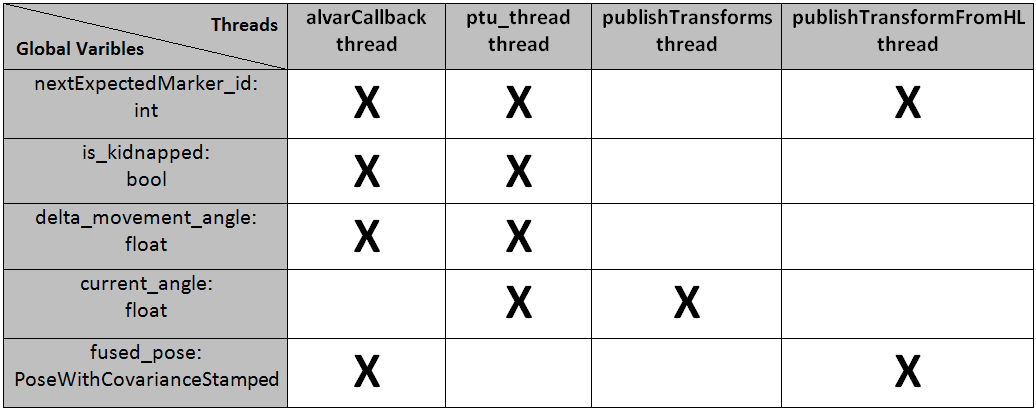
\includegraphics[width = \linewidth]{graphics/vision_threads.png}
\caption{Thread Communication}
\label{Thread Communication}
\end{center}
\end{figure}



\section{Problems and Challenges}

As already mentioned, there were as usually a lot problems practically from the start. But all of them are successfully resolved now and we have learned a lot from them. Here some of the problems we had will be briefly shown. First problem that we confronted was the wrong setup of the ar\_track\_alvar launch file, it wasn’t meant to work with freenect\_launch, so we had to change the start connection between nodes, so that ar\_track\_alvar gets data from the Kinect. Next problem, that we found by computing the covariance, was that the values we got from the algorithm were too inaccurate. We solved this problem by finding and implementing queue with the right size of 25 samples, so that program have enough data in order to give back the right covariance. After that we spent time thinking about size of the marker, so that we can maximize distance from which Kinect will be able to see the marker. We tried bundles of markers, i.e. two and three markers on one, tried single marker and then stopped with this solution. Then we worked on a problem of positioning markers on the map (i.e. in the building), so that they are not too far away from each other and on the other hand so that there are not too much of them on the map. Because otherwise it would be irritating for the robot to see two markers at the same time. That problem was found while implementing an algorithm for the next expected marker. Then, working with PTU we had a problem finding a right procedure to turn towards the expected marker, $atan$ had cases where it wasn't defined, so at the end we used $atan2$, because it considers all the special cases. Afterwards we had a problem with stopping the head when it was already looking in the markers direction. We solved it by lowing accuracy of the marker following. One of the last problems were the axes, that were not parallel to each other. We saw it in rviz and needed to dive into the code once again to find an error. Error consisted in the wrong implementation of database. As we changed it, everything was working fine. 

\section{Testing}

Our first test was to find out how far the robot can go, so the marker is still being recognized. We found out that the viewing angle is approximately 58 degrees and viewing distance is 3.4 meters.
 After that we decided to put every marker on the wall within 2,5 meter distance. It turned out to be a pretty good result. Then we worked on PTU movement to find out the right speed, so that it won’t turn neither too slow or too fast. We found out that 0,7 radians per second is exactly what we need. Besides that we wrote a dummy program to check if all values are interpreted as we need. As we ended up testing our software, we were practically done with our part of the project.

\begin{figure}
\begin{center}
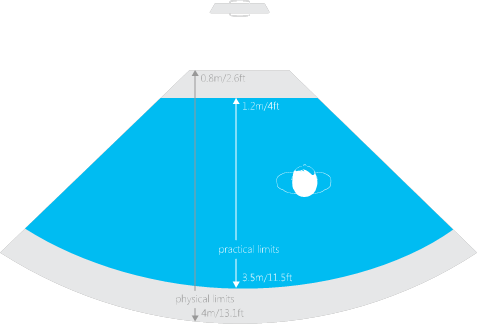
\includegraphics[scale=0.8]{graphics/view_field.png}
\caption{Field of View}
\label{Field of View}
\end{center}
\end{figure}
